\cotefile{34}
\scanpage{165}
\mspage{2}
% archive sheet number: 164
un \unsure{automorphisme} intérieur de $\pi^{\unsure{(p')|(p)}}$, donc induit un homomorphisme de gpes profinis
\[
\operatorname{Aut\,\unsure{Ext|ext}}(\pi)\longrightarrow\operatorname{Aut\,ext}(\pi^{(p')})
\tag*{(1.1.1)}
\]

\deleted{En particulier, si $\pi=\pi_1(X_{\bar K},\xi)$, \unsure{on a} \illegible{1}}
Soit en particulier $\unsure{X_\eta|X_K}$ un schéma géom. connexe sur $K$, \deleted{\unsure{$K$}} muni d'un pt géom. $\xi$, et $\bar K$ la clôture \unsure{sép|sep} de $K$ dans $k(\xi)$ [de sorte que $\xi$ ``est'' un pt géom. de $X_{\bar K}$]. On a une suite exacte (SGA 1 IX 6.1)
\[
1\to\pi_1(X_{\bar K},\xi)\mathrel{\text{---}}\pi_1(X,\xi)\longrightarrow
\underset{\underset{I}{\Vert}}{\operatorname{Gal}(\bar K/K)}\mathrel{\text{---}}1
\tag*{(1.1.2)}
\]
qui définit donc un homomorphisme
\[
I\longrightarrow\operatorname{Aut\,ext}\,\pi_1(X_{\bar K},\xi).
\tag*{(1.1.3)}
\]
Soit $\pi_1(X,\xi)'$ \deleted{\unsure{le sous}} \inserted{le} -groupe quotient de $\pi_1(X,\xi)$ par le sous-groupe \deleted{\unsure{fermé}} \inserted{fermé} engendré par les $p$-sous-groupes de Sylow de $\pi_1(X_{\bar K},\xi)$, on trouve donc une suite exacte
\[
1\mathrel{\text{---}}\pi_1(X_{\bar K},\xi)^{(p')}\mathrel{\text{---}}\pi_1(X,\xi)'\mathrel{\text{---}}
\underset{\underset{I}{\Vert}}{\operatorname{Gal}(\bar K/K)}\mathrel{\text{---}}1,
\tag*{(1.1.4)}
\]
qui définit un hom.
\[
I\mathrel{\text{---}}\operatorname{Aut\,ext}\,\pi_1(X_{\bar K},\xi)^{(p')},
\tag*{(1.1.5)}
\]
qui n'est autre que le composé de (1.1.1) et (1.1.3).
\scanpage{166}
\mspage{3}
% archive sheet number: 165
Dans la suite, on se propose de donner des renseignements sur (1.1.5) lorsque $X$ est de type fini sur $K$, $K$ étant un ``corps local'' comme à l'accoutumée\unsure{...}

1.2. Lorsque le \deleted{\illegible{2}} pt géom. $\xi$ de $X_K$ est localisé en un point rationnel sur $X$, alors la suite exacte (1.1.2) \unsure{splitte|splite} canoniquement, et \deleted{\unsure{que}} on peut écrire $\pi_1(X,\xi)$ comme un produit $\frac12$ direct
\[
\pi_1(X,\xi)\simeq\pi_1(X_{\bar K},\xi).I,
\tag*{(1.2.1)}
\]
moyennant une action de $I$ sur $\pi_1(X_{\bar K},\xi)$ :
\[
\deleted{\unsure{I\mathrel{\text{---}}}}\quad I\mathrel{\text{---}}\operatorname{Aut}(\pi_1(X_{\bar K},\xi)).
\tag*{(1.2.\unsure{2|4})}
\]
\unsure{De même on aura|De même aussi on a}
\[
\pi_1(X,\xi)'\simeq\pi_1(X_{\bar K},\xi)^{\unsure{(p')|(p)}}.I,
\tag*{(1.2.\unsure{3|8})}
\]
moyennant un hom.
\[
\deleted{\unsure{\pi}}I\mathrel{\text{---}}\operatorname{Aut}(\pi_1^{(p')}(X_{\bar K},\xi)).
\tag*{(1.2.4)}
\]
composé de \unsure{1.1.7|1.1.2} et l'hom de fonctorialité
\[
\operatorname{Aut}\pi_1\mathrel{\text{---}}\operatorname{Aut}\pi_1^{(p')}.
\]

\deleted{\unsure{Lem}} \unsure{Explicitons|Expliciter} ici la suite exacte, valable pour tt gpe profini $\pi$
\[
1\mathrel{\text{---}}\pi/\unsure{z|Z}\mathrel{\text{---}}\operatorname{Aut}(\pi)\longrightarrow\operatorname{Aut\,ext}\pi\deleted{^{\unsure{(p')}}}\mathrel{\text{---}}1
\qquad \{Z=\text{centre de }\pi.
\tag*{(1.2.5)}
\]
Appliquée au cas de $\pi_1^{(p')}$, cette suite nous montre ceci :
\scanpage{167}
\mspage{4}
% archive sheet number: 166
% A vertical emphasis line stands at the left of the lemma and its parenthesis.
\uline{Lemme} 1.2.6. Pour que l'opération \inserted{(1.2.4)} du groupe d'inertie $I$ sur $\pi_1^{\unsure{(p')|(p)}}(X_{\bar K},\xi)\deleted{^{\unsure{(p)}}}$ soit ``\uline{modérément} ramifiée'' i.e. pour que l'image \inserted{de $I$ dans $\operatorname{Aut}\pi_1^{(p')}(X_{\bar K},\xi)$} soit un gpe profini \uline{premier à $p$}, il \unsure{f. et s.} qu'il en soit ainsi de l'image de $I$ dans $\operatorname{Aut\,ext}(\pi_1^{(p')}(X_{\bar K},\xi))$ (via (1.1.5)). En particulier, cette condition ne dépend pas du choix du point \deleted{\unsure{géom. $\xi$}} choisi de $X_K(K)$.

\deleted{\unsure{Si cette condition est}}
\deleted{On dit alors, par abus de}
(Si cette dernière condition est satisfaite, on dit aussi que $I$ \uline{opère modérément} (sous-entendu : mod. aut. intérieurs) sur $\pi_1^{(p')}(X_{\bar K},\xi)$.)

Ceci posé, nous avons en vue la démonstration des deux résultats principaux :

% slanted
\margin{\deleted{\illegible{5} \unsure{d'un cas}}}
\uline{Théorème} 1.3. \inserted{(Théorème de l'action essentiellement modérée du groupe de monodromie \inserted{locale})}
Soit $X$ de type fini sur \deleted{\unsure{le corps}} $K$, $\xi$ un pt géom de $X$, $\bar K$ la clôture séparable correspondante de $K$, d'où $I=\operatorname{Gal}(\bar K/K)$ opérant \inserted{``extérieurement''} sur $\pi_1^{(p')}(X_{\bar K},\xi)$.
\deleted{\unsure{il existe un sous-groupe}}
\inserted{Alors (pour mémoire) $\pi_1^{(p')}(X_{\bar K},\xi)$ est} topologiquement \deleted{à engendrement} \inserted{de type} fini, et \deleted{\unsure{il}} il existe un sous-groupe ouvert $I'$ de $I$ qui opère \uline{modérément} (1.2.6) sur $\pi_1^{(p')}(X_{\bar K},\xi)$.

\uline{Remarque} 1.3.1. En fait, utilisant le résultat précédent, \inserted{(ou au choix le résultat 1.4 dans le cas de la dim. relative 1)} \deleted{\unsure{la théorie relative}} \inserted{et la résolution des singularités dans le cas non propre,} un argument dû à J. P. Murre (SGA 1 \uline{XIII}) permet de prouver ceci : Soit $X$ de t. f. sur $k$ sép clos, \deleted{$\xi$ un pt de \unsure{car.}} d'exp. car. $p$, $\xi$ un pt géom
\scanpage{168}
\mspage{5}
% archive sheet number: 167
de $X$. Alors $\pi_1^{\unsure{(p')|(p)}}(X,\xi)$ est (en tant que \unsure{pro-$p'$-groupe|pro-fini-groupe}) de présentation finie.

\uline{Th. 1.4} (Th. de l'action modérée du groupe de monodromie locale). Soient $S$ un schéma strictement local, $\bar X$ un schéma sur $S$, $Y$ un sous-schéma fermé de $\bar X$, $X=\bar X-Y$.
\inserted{$U$ un ouvert de $S$ (resp. $\eta$ un pt de $U$), $\xi$ un pt géom. de $X|U$ (resp. de $X_\eta$). \deleted{\unsure{On suppose}} Dans le cas non resp., $\eta$ désigne le pt de $S$ sous $\xi$.}

a) $\bar X$, \inserted{$Y$} \deleted{sont} projectifs, de présentation finie, \deleted{\unsure{plats}} sur $S$, \inserted{l'ens des pts de $\bar X_s$ \unsure{où} $\bar X$ ou $Y$ n'est pas plat sur $S$ est de codim $\geq2$ dans $\bar X_s$.}

\deleted{b) L'ensemble des pts de $\unsure{X_s|Y_s}$ \unsure{de} \illegible{4} de codim $\geq2$ dans $\bar X_s$, et} $Y_s$ est rare dans $\bar X_s$.

c) $\bar X_s$ est, dans le complémentaire d'une partie de codim $\geq2$, un ``\deleted{diviseur}\inserted{schéma} à croisements normaux''.
\deleted{\unsure{Les fibres}} \deleted{\unsure{les pts de}} \deleted{$\bar X_\eta$ \unsure{est géométriquement} \illegible{2} \unsure{non lisse} \illegible{2} \unsure{la fibre est} $\geq2$ \unsure{(resp. $\bar X_\eta$)}}

% slanted
\margin{\deleted{\unsure{tout ceci} \illegible{3} \unsure{par une} \illegible{3}}}
% slanted
\margin{\unsure{Remplacer} l'ouvert $U$ ou le point $\eta$ par un schéma $T$ géom connexe sur $S$, avec hypothèse assurant que $I=\pi_1(T,\xi)$ opère sur $\pi_1^{(p')}(X_{\bar\eta},\xi)$.}

d) $\bar X|U$ est lisse et $Y|U$ diviseur à croisements normaux relatifs (resp. $\bar X_\eta$ a un ens de non-lissité de codim $\geq2$).
\deleted{De plus, $\bar X_\eta$ est \unsure{géométriquement} \illegible{2}, et $Y_\eta$ est \unsure{fini}.}
\inserted{$\bar X_{\bar\eta}$ est \deleted{géom intègre} irréductible.}

Soit $I=\pi_1(U,\xi)$ [resp. $I=\pi_1(\eta,\xi)\{=\operatorname{Gal}(\bar\eta/\eta)\}$], considérons l'hom naturel
\[
I\mathrel{\text{---}}\operatorname{Aut\,ext}\,\pi_1^{(p')}(X_{\bar\eta\deleted{\unsure{\bar K}}},\xi)
\]
\deleted{resp. $I\mathrel{\text{---}}\operatorname{Aut\,ext}\,\pi_1^{(p')}(X_{\bar\eta},\xi)$}

\diagram{\begin{tikzcd}[ampersand replacement=\&]
\bar X \arrow[d,no head] \& \bar X|U \arrow[d,no head] \& \xi \arrow[l,no head] \\
S \& U \arrow[l,hook'] \&
\end{tikzcd}}
Lorsque l'on se donne une section $g$ de $\bar X$ sur $S$ contenue dans l'ouvert de lissité, on trouve de même un hom
\[
I\mathrel{\text{---}}\operatorname{Aut\,ext}(\pi_1^{(p')}(X_{\bar\eta},\xi))
\]
Ceci posé, l'image de l'un et l'autre hom. est un \uline{groupe \unsure{abélien} commutatif premier à $p^{\unsure{=|'}}$}.

Si $\bar X$ est de dim relative 1 sur $S$, alors \deleted{\unsure{la fin}} rang \inserted{topologique} du groupe image est $\leq\unsure{\nu|v}$, où $\nu$ est le nb de pts singuliers de $X_{\bar s}$.
\scanpage{169}
% archive sheet number: 168
\deleted{\uline{Exercice} 7.8. (\uline{Topos locaux.})}
% The remaining faint, reversed marks are show-through from the other side.
\scanpage{170}
\mspage{6}
% archive sheet number: 169
2. \uline{Réduction à un cas \unsure{standard|standart} de dim. relative 1}.

\deleted{La réduction de 1.3. Au cas où $X$ est lisse sur $K$, de dim relative 1 se fait suivant les lignes de la réduction analogue faite dans II 3, du moins}

2.1. \uline{Réduction de 1.3 au cas} $X$ \deleted{\unsure{affine géom.}} \deleted{\unsure{géométriquement projectif}} \deleted{\uline{géom. et normal}} \inserted{\deleted{\unsure{affine}} \uline{géométriquement normal et géom intègre}}

\deleted{On recouvre $X$ par des ouverts affines $X_i$}
\deleted{2.1.1. Réduction au cas $X$ affine}
\deleted{en nb fini, on pose $X'=\coprod_i X_i$, $X''=X'\mathbin{\times}_X X'$, $X'''=X'\mathbin{\times}_X X'\mathbin{\times}_X X'$.}

\deleted{\unsure{Soit} $X$} Notons que l'on peut \deleted{\unsure{supposer provisoirement}} \inserted{supposer $S$} complet (I\quad), et qu'il est inoffensif pour la conclusion de remplacer $V$ par \unsure{sa|son} normalisé dans une extension finie $K'$ de $K$, et $X_K$ par $X_{K'}=X_K\otimes_K K'$ (car cela revient à remplacer $I$ par un s-groupe ouvert $I'$).
On peut alors, quitte à passer à une extension radicielle $K'$ de $K$, supposer que \deleted{\unsure{$X$}} le normalisé \deleted{\unsure{de}} de $(X_K)_{\mathrm{red}}$ est \uline{géométriquement normal} (EGA \uline{IV} \unsure{17.11.14.2|17, II.14.2}).
\deleted{De plus (EGA IV 4) on peut supposer $X_K$ géom. connexe. Enfin}

% slanted
\margin{\unsure{on est ramené} au cas où le pt de base sur $X_K$ est un $x\in X_K(K)$}
Soit $X_0$ le normalisé de $X_{\mathrm{red}}$ et soient $X_1$ et $X_2$ ses produits fibrés \inserted{sur $X$}. Dans SGA 1 IX 5, nous avons donné une méthode à la Van Kampen pour calculer le groupe fondamental de $X$ par générateurs et relations en termes de ceux des \inserted{comp. connexes des} $X_0,X_1,X_2$. Nous pouvons d'ailleurs supposer, quitte à faire une ext. finie sur $K$, que ces comp. connexes sont géom. connexes (EGA IV 4). \deleted{Alors le groupe fondamental} \inserted{\unsure{Nous pouvons aussi}} supposer que les pts bases choisis dans ces comp. \unsure{supposées|sont}
\scanpage{171}
% archive sheet number: 170
% Four long diagonal cancellation strokes cross the working sheet.
\deleted{$X_1\qquad X_2$}
\diagram{\begin{tikzcd}[ampersand replacement=\&,column sep=small]
\deleted{X'''} \arrow[d,shift left=1.4pt,no head] \arrow[d,no head] \arrow[d,shift right=1.4pt,no head] \& \deleted{\pi_0(X''')} \\
\deleted{X''} \arrow[d,shift left=.8pt,no head] \arrow[d,shift right=.8pt,no head] \& \deleted{\pi_0(X'')} \\
\deleted{X'} \arrow[d,no head] \& \deleted{\pi_0(X')}\quad\text{\deleted{\uline{un seul pt}}} \\
\deleted{X} \&
\end{tikzcd}}

\diagram{\begin{tikzcd}[ampersand replacement=\&]
\deleted{\pi_1(X',\bar x)} \arrow[d] \\
\deleted{\pi_1(X,\bar x)}
\end{tikzcd}}
\deleted{$P\subset I$ \unsure{opère} \unsure{triv\textsuperscript{t}|trivialm.} sur $\pi_1(X',\bar x)$ donc sur son \unsure{image}.}

\figure{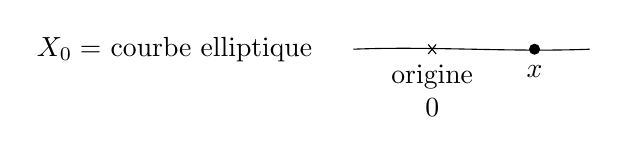
\begin{tikzpicture}
\node[anchor=east] at (-.4,0) {\deleted{$X_0=$ courbe elliptique}};
\draw (0,0) .. controls (1,.04) and (2,-.04) .. (3,0);
\draw (.95,-.06)--(1.05,.06) (.95,.06)--(1.05,-.06);
\fill (2.3,0) circle (2pt);
\node[below,align=center] at (1,-.08) {\deleted{origine}\\\deleted{$0$}};
\node[below] at (2.3,-.08) {\deleted{$x$}};
\end{tikzpicture}}
\figure{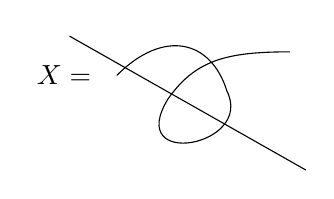
\begin{tikzpicture}
\node[anchor=east] at (-.2,0) {\deleted{$X=$}};
\draw (0,0) .. controls (.6,.6) and (1.2,.45) .. (1.4,-.2)
.. controls (1.75,-.9) and (.1,-1.2) .. (.65,-.3)
.. controls (1,.2) and (1.4,.3) .. (2.2,.3);
\draw (-.6,.5)--(2.4,-1.2);
\end{tikzpicture}}
\[
\deleted{H^0(K,A)\longrightarrow H^1(K,T_\ell(A))}
\]

\diagram{\begin{tikzcd}[ampersand replacement=\&,column sep=small,row sep=large]
\deleted{X} \arrow[dd] \& \deleted{X_K} \arrow[l] \arrow[dd] \& \& \deleted{X_{\unsure{\widetilde U|\widetilde\eta}}} \arrow[ll] \arrow[dd,no head] \& \\
\& \& \deleted{X} \arrow[ul] \arrow[dd,no head] \& \& \deleted{\widetilde X} \arrow[ul] \arrow[ll] \arrow[dd,no head] \quad \deleted{\unsure{F_{\bar a}|F_{\bar\alpha}}} \\
\deleted{S} \arrow[uu,bend left=20] \& \deleted{U} \arrow[l,hook'] \arrow[uu,bend left=20] \& \& \deleted{\bar U} \arrow[ll] \& \\
\& \& \deleted{S} \arrow[ul] \& \& \deleted{\bar S} \arrow[ll] \arrow[ul]
\end{tikzcd}}

\diagram{\begin{tikzcd}[ampersand replacement=\&]
\deleted{\unsure{\mathscr B|B}_{\unsure{\Gamma|\mathscr T|T}}} \arrow[d] \& \deleted{\mathscr B_\pi} \arrow[l] \arrow[d] \& \\
\deleted{\unsure{P|p}} \& \deleted{\mathscr B_I} \arrow[l] \& \deleted{P} \arrow[l]
\end{tikzcd}}
\scanpage{172}
\mspage{7}
% archive sheet number: 171
connexes \unsure{sont|soient} les pts géom. déduits (via l'extension fixée $\bar K$ de $K$) de pts $x_{i\alpha}$ $(i=0,1,2)$ \deleted{des} \uline{rationnels} /$K$.
On utilise loc. cit. pour déterminer $\pi_1(X^c_{\bar K},\xi)$ comme gpe engendré par \inserted{les} $\pi_1(X^c_{0\bar K},\xi_0^c)$ et des générateurs $\unsure{g_{c'}|\gamma_{c'}}$ (indexés par l'ens des composantes connexes de $X_1$, soumis à des relations qui ne nous importent pas ici.
\deleted{Le choix \inserted{particuliers faits} des pts bases \unsure{implique}}

\deleted{Il suffira que} Cette description est canonique en dehors du choix de \deleted{\unsure{certains}} ``classes de chemins'' reliant des pts géométriques \inserted{$\bar a,\bar b$} d'une même composante connexe \inserted{$X^c_{0\bar K}$} de $X_{0\bar K}$, \deleted{\unsure{le}} [savoir le pt marqué de $X^c_{0\bar K}$ et l'image d'un pt marqué d'un $X^{c'}_{1\bar K}$ par l'une ou l'autre projection.
\deleted{\unsure{Le choix des}}
\deleted{Alors les \unsure{faits décrits ci-dessus}}
Plus précisément, on doit faire le choix d'un isom entre les foncteurs fibres $F_{\bar a},F_{\bar b}$ associés à $\bar a,\bar b$ sur la catégorie $\operatorname{Rev\,ét}(X^{\unsure{c'|c}}_{0\bar K})$ des rev. étales de $X^c_{0\bar K}=:Y_{\bar K}$.
\inserted{par construction, $\bar a,\bar b$ proviennent de pts \deleted{\unsure{géom. de $X$} $\unsure{\xi}(K)$, de} $a,b\in Y_K(K)$}
\deleted{\unsure{Au}} \unsure{Le} groupe d'inertie $I=\operatorname{Gal}(\bar K/K)$ opère par
\deleted{suite sur les foncteurs fibres $F_{\bar a},F_{\bar b}$ [donnant naissance aux opérations de $I$ sur $\pi_1(X^{c'}_{1\bar K},\bar a)$ et $\pi_1(X^{c'}_{1\bar K},\bar b)$}
\deleted{Ceci dit, on peut choisir les isom $F_{\bar a}\simeq F_{\bar b}$ de façon à commuter à l'action de \deleted{\unsure{\pi}} $I$}
sur l'ens \deleted{couples}
\[
\deleted{(\operatorname{Rev\,ét}(Y_{\bar K}),F_{\bar a}),
(\operatorname{Rev\,ét}(Y_{\bar K})F_{\bar b})}
\]
\unsure{des} ``classes de chemins'' de $\bar a$ à $\bar b$, \deleted{Nous admettrons} \inserted{qui est} \inserted{un torseur sous $\pi_1(Y_{\bar K},\bar a)$}, à groupe d'opérateurs $I$ [compatible \deleted{\unsure{avec les homomorphismes}} avec les opérations de $I$ sur les $\pi_1$).

% Cancellation scribble in the lower left margin.
\deleted{\uline{Lemme} 2.1.1. \unsure{Il existe|Soit} $Y_K$ de type fini géom connexe sur $K$, muni de $a,b\in Y_K(K)$, alors $I$ opère sur l'ens \inserted{$P$} des classes de chemins de $\bar a$ en $\bar b$ sur $Y_{\bar K}$. Ceci posé}
\scanpage{173}
\mspage{8}
% archive sheet number: 172
Il n'est pas vrai en général que \deleted{\unsure{toujours}} ce torseur à opérateurs $I$ soit trivial, i.e. admette un élément invariant par $I$;
\deleted{Mais si $P$ est le groupe de Sylow, on}
\inserted{l'obstruction est dans un $H^1(I,\pi_1(Y_{\bar K},\bar a))$}
($\unsure{H^1|H}$ non commutatif). Mais considérons le \deleted{\unsure{$p$}} torseur $Q^{\unsure{(p')|(p)}}$ associé de groupe \deleted{$\unsure{R|K}$} structural (à opérateurs $I$) $\pi_1^{(p')}(Y_{\bar K},\bar a)$, et la restriction des $I$-opérations au s-groupe $P\subset I$ ($p$-sous-groupe de Sylow). Je dis qu'il existe un élément de $Q^{(p')}$ fixe sous $P$, i.e. que la classe $c^{(p')}|P\in H^1(P,\pi_1^{(p')}(Y_{\bar K},\bar a))$ est nulle : Ceci provient en effet du fait que $P$ est un $p$-groupe et \inserted{$G:$} $\pi_1^{(p')}(Y_{\bar K},\bar a)$ est premier à $p$ : à prouver que \deleted{\unsure{toute}} toute section multiplicative $\varphi$ du produit $\frac12$ direct $G.I\to I$ est conjuguée de la section \unsure{standard|standart} par un élément de $G$. Or par le th de \inserted{conjugaison} Sylow, il existe un élément $g.i\in G.I$ tel que $\operatorname{int}(g.i)I=\varphi(I)$, i.e. $\operatorname{int}(g)I\subset\varphi(I)$, d'où la conclusion.
\scanpage{174}
\mspage{9}
% archive sheet number: 173
\deleted{il existe un élément \unsure{$x\in P$} $\gamma\in P$ \unsure{qui} dont le groupe de stabilité dans $I$ est ouvert.}

Ceci posé, nous pouvons supposer \unsure{choisis|choisies} des ``classes de chemins'' dans \inserted{le th. de} ``Van Kampen'', \deleted{\unsure{pour}} \inserted{où les $\pi_1$ remplacés par $\pi_1^{\unsure{(p')|(p)}}$} de telle façon qu'ils soient invariants par $P$. \deleted{quitte à passer à une extension finie de $K$.} Alors, on voit par ``transport de structure'', que \deleted{\unsure{le groupe}} l'hom
\diagram{\begin{tikzcd}[ampersand replacement=\&,column sep=small]
\Pi^{(p')} \arrow[d] \& =\text{gpe \inserted{profini premier à $p$} engendré par les }\pi_1^{(p')}(X^c_{0\bar K},\bar x_{0\alpha})\text{ et les }g_{c'} \\
\pi_1^{(p')}(X_{\bar K},\bar x) \&
\end{tikzcd}}
est compatible avec l'action de $I$, quand $I$ opère sur $\Pi$ via les opérations naturelles de $I$ sur les $\pi_1^{(p')}(X^c_{0\bar K},\bar x_{0\alpha})$ (1.2), et l'opération \uline{\unsure{triviale|trivial}} sur \inserted{les} $g_{c'}$.

\deleted{De ce fait l'hom correspondant}
\[
\deleted{\Pi^{(p')}\mathrel{\text{---}}\pi_1^{(p')}(X_{\bar K},\bar x)}
\]
\deleted{est compatible avec les opérations de $I$. Ceci dit, si $P$ est le $p$-ss-groupe de Sylow de $I$}
Si on sait que $P$ opère trivialement sur les $\pi_1^{(p')}(X^c_{0\bar K},\bar x_{0\alpha})$, il opère aussi trivialement sur $\Pi^{(p')}$ qui est engendré par des invariants et par les $g_{c'}$ fixes \deleted{\unsure{par $I$}} par $P$, donc $P$ opère trivialement sur \deleted{le quotient $\pi_1^{(p')}$} $\pi_1^{(p')}(X_{\bar K},\bar x)$, puisque \unsure{$\alpha$|cet hom} est \uline{surjectif}. Donc on est ramené \deleted{\unsure{on}} à prouver 1.3 pour les $X_0^c$ au lieu de $X$, donc on peut supposer $X$ \deleted{\unsure{géom. et|géom. intègre}} \inserted{géom.\textsuperscript{t}} normal.
\scanpage{175}
\mspage{10}
% archive sheet number: 174
2.2. \uline{Réduction de} 1.3 \uline{au cas} $X$ \deleted{géom.} \uline{affine lisse de dim 1}.

Soit $U_K$ un ouvert affine \deleted{\unsure{connexe|non vide}} de $X_K$, \deleted{Alors} contenant le pt \deleted{base géom.} $x$. Alors $\pi_1'(U_{\bar K},\bar x)\mathrel{\text{---}}\pi_1(X_{\bar K},\bar x)$ est surjectif et compatible avec les op. de $I$, donc de même pour $\pi_1^{\unsure{(p')|(p)}}(U_{\bar K},\bar x)\mathrel{\text{---}}\pi_1^{(p')}(X_{\bar K},\bar x)$, donc on est ramené au cas de $X$ affine, a fortiori quasi-projectif. La réduction \inserted{au cas} où de plus $\dim X=1$ se fait alors à coups de sections hyperplanes génériques, comme en II 3. \deleted{\unsure{Comme}}

2.3. \uline{Réduction de} 1.3 \uline{au cas de la situation 1.4, avec} \deleted{\illegible{1}} $\uline{\dim} X_K=1$.
\inserted{En vertu de I, on peut supposer \unsure{maint.|normal} $S$ complet.}
Considérons le modèle complet $\bar X_K$ de $X_K$. Quitte à faire une extension radicielle de $K$, on peut supposer $\bar X_K$ géom. normal, i.e. lisse.
De plus, un théorème non trivial, qui sera vu dans un exposé ultérieur (\quad), nous apprend que, quitte à \deleted{\unsure{remplacer}} passer à une extension finie de $K$, il existe un \deleted{\unsure{mod}} schéma projectif $\bar X$ sur $S$, ayant $\bar X_K$ comme fibre générique, et tel que $\bar X_s$ soit \deleted{géométriquement réduit} un diviseur à croisements normaux dans $\bar X$, $X_s$ étant de plus réduit et son normalisé étant \deleted{géom.} \uline{lisse} sur $\unsure{K|k}$.

\margin{corps résiduel parfait ? Mais on s'y ramène pour prouver 1.3, \deleted{\unsure{déjà fait}} \inserted{par réduction} à un ss groupe \deleted{\unsure{distingué}} \inserted{ouvert} de $I$, cf I\unsure{...}}

Agrandissant encore $K$, on peut supposer que les pts de $\bar X_K-X_K$ sont rationnels sur $K$, donc \inserted{($\bar X$ étant propre sur $S$)} sont définis par des sections $g_i$ de $\bar X$ sur $S$, $1\leq i\leq r$. La réduction est
\scanpage{176}
\mspage{11}
% archive sheet number: 175
terminée si \deleted{nous prouvons que} \inserted{les $g_i(S)$} sont mutuellement disjointes et contenues dans l'ouvert de lissité de $\bar X$ sur $S$.
\deleted{\unsure{Il faut donc le} cas contraire, il faut examiner les ennuis qui peuvent se présenter : 1) \unsure{$g_i(s)$} $\exists i$ tel que $g_i(s)$ soit un pt double de $X_s$. Faisant éclater}

\figure{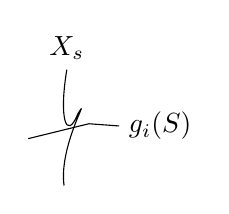
\begin{tikzpicture}[scale=.7]
\draw (0,-1) .. controls (-.1,-.3) and (.5,.7) .. (.25,.3)
.. controls (.05,-.2) and (-.1,.2) .. (.05,1.1);
\draw (-.65,-.15)--(.45,.12)--(1,.08);
\node[above] at (.05,1.1) {$X_s$};
\node[right] at (1,.08) {$g_i(S)$};
\end{tikzpicture}}

Mais si $D$ est le diviseur $X_s+\sum g_i(S)$ sur le schéma régulier $\bar X$, on sait (\quad) que, quitte à faire éclater un nb fini de fois des pts fermés de $\bar X$ (qui sont nécessairement dans $\bar X_s$, donc le processus ne touche pas à $\bar X_K$, \deleted{\unsure{ni}} à fortiori à $X_K$), on peut supposer que $D$ est à \uline{croisements normaux}. Mais ceci implique que les $g_i(S)$ sont mutuellement disjoints (sinon on aurait
\figure{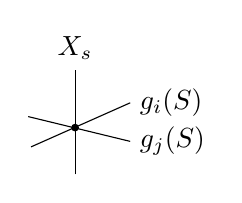
\begin{tikzpicture}[scale=.7]
\draw (0,-.8)--(0,1.1);
\draw (-.8,-.3)--(1,.5);
\draw (-.85,.25)--(1,-.2);
\fill (0,.05) circle (2pt);
\node[above] at (0,1.1) {$X_s$};
\node[right] at (1,.5) {$g_i(S)$};
\node[right] at (1,-.2) {$g_j(S)$};
\end{tikzpicture}}
, \deleted{\unsure{contraire}} qui n'est pas à croisements normaux).
\deleted{et que $g_i(S)\cap X_s=\{g_i(s)\}$ est un pt de lissité de $X_s$ (sinon on aurait}
\figure{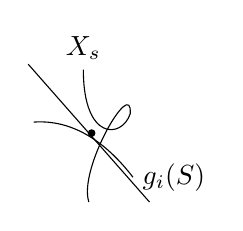
\begin{tikzpicture}[scale=.7]
\draw (0,-1) .. controls (-.2,-.4) and (.8,1.3) .. (.75,.6)
.. controls (.6,.15) and (-.1,.1) .. (-.1,1.4);
\draw (-1,.45) .. controls (-.3,.5) and (.3,.1) .. (.8,-.55);
\fill (.05,.25) circle (2pt);
\node[above] at (-.1,1.4) {\deleted{$X_s$}};
\node[right] at (.8,-.55) {\deleted{$g_i(S)$}};
\draw (-1.1,1.5)--(1.1,-1);
\end{tikzpicture}}
\deleted{). Enfin}
\inserted{D'autre part,} comme $X$ est \uline{régulier}, chaque section $g_i$ de $X$ sur $S$ est dans l'ouvert de lissité de $X$ (EGA IV 17\unsure{..}). La réduction de 1.3 au cas 1.4 est achevée.

\deleted{2.4. \uline{Réduction de 1.4 au cas de la dim. relative 1}, \unsure{projectif}}
\deleted{\unsure{prenons le} \illegible{2} \unsure{projectif} \illegible{2} de $S$ \illegible{2}}
\deleted{\inserted{Pour ceci, on peut supposer $X$ géom connexe de dim $n\geq2$} \unsure{Choisissons un} \illegible{1} et le th. prouvé en dim relative $<n$.}
\deleted{$\bar X\subset\mathbb P_S^r$, d'où $\bar X_s\subset P_s^r$. Soit $Z_s$ le normalisé de $\bar X_s$, de sorte qu'on a un morphisme \unsure{nat.|net}}
\[
\deleted{Z_s\longrightarrow P_s^r\quad\text{(EGA V)},}
\]
\deleted{$Z_s$ étant lisse \inserted{de dim $n$} \unsure{géométriquement}. On sait alors que pour un \deleted{\unsure{seul}} hyperpl ``assez général'' $H_s$ de $P_s^r$, $Z_s\mathbin{\times}_{\mathbb P_s^r}H=Z'_s$ est \unsure{connexe}}
\scanpage{177}
\mspage{12}
% archive sheet number: 176
% slanted
\margin{Il suffit de prouver l'énoncé relatif au cas où on a une section, grâce à a), b) et \unsure{Bertini|Recours|Zariski} \unsure{au pluriel}\unsure{...}}
2.4. \uline{Réduction de 1.4 au cas de la dim relative 1}.
Supposons la dim relative $n\geq2$, et le th. \uline{prouvé} en dim relative $n-1$.
Choisissons une immersion de $\bar X$ dans $P_S^r$. \deleted{Choisissons} On peut supposer que la section $g$ est de coordonnées $(1,0,\ldots,0)$. On \inserted{considère} le schéma \deleted{\unsure{strict}} $S'$ localisé strict de $S[\unsure{t_0|t_1},\ldots,t_r]$ au pt maximal de la fibre spéciale, et les images inverses \deleted{\unsure{$\xi$}} $\bar X',Y',X',U'$ sur $S'$. On peut relever $\xi$ en un pt géom de $\bar X'$, \deleted{également} noté $\xi'$, dont l'image dans $S'$ \deleted{est} est notée $\eta'$.
\inserted{On peut supposer $\eta'$ générique dans la fibre de $S'$ sur $\eta$.}

\diagram{\begin{tikzcd}[ampersand replacement=\&]
\& \unsure{\xi|\xi'} \arrow[d] \\
\bar X \arrow[d,no head] \& \bar X' \arrow[l,no head] \arrow[d,no head] \\
S \& S' \arrow[l]
\end{tikzcd}}

\deleted{Dans le cas non resp., on désigne par $U'$ \unsure{l'ouvert|l'image} de $S'$ formé des pts $t$ au dessus de $U$ en lesquels la fibre $\bar X'_t$ est lisse et $Y'_t$ est un diviseur à croisements normaux.}
Considérons \inserted{(quitte à agrandir $k(\xi')$)} l'hyperplan $H\subset P_{S'}^r$ ``générique'' \inserted{passant par $g$} relativement à $S$, de coordonnées $(\unsure{0|t_0},t_1,\ldots,t_r)$. \deleted{Alors \unsure{Posons}} Alors \deleted{Dans le cas non resp., on désigne par $U'$ l'ouvert de} \deleted{considérons le plus grand ouvert de $S$ au dessus duquel}
\[
\bar X^{(1)}=\bar X'\cap H\quad\text{et}\quad Y^{(1)}=Y'\cap H
\]
sont \inserted{projectifs et} plats sur $S$, de présentation finie sur $S$, \deleted{Soit $V'$ l'aire de \unsure{$s$}} \inserted{donc $(\bar X^{(1)},Y^{(1)},X^{(1)}=\bar X^{(1)}-Y^{(1)})$ est} \deleted{la condition} satisfait la condition a). Ils satisfont aussi les conditions b) et c) (\deleted{\unsure{immédiat de}} réf : EGA V).

% slanted
\margin{On peut être obligé de remplacer l'immersion projective envisagée par \unsure{un multiple|une multiple} (le carré doit suffire).}
Dans le cas resp., on peut choisir $\xi'$ de façon que $\eta'$ soit gén. dans la fibre de $S'$ sur $\eta$, alors d) sera satisfaite pour $\bar X^{(1)}_{\eta'}$. Dans le cas non resp., \deleted{\unsure{on}} je dis que si $U'$ est le plus grand ouvert de $S'|U$ \deleted{sur lequel} \inserted{tel} que $\bar X^{(1)}|U'$ soit lisse sur $U'$ et $Y^{(1)}|U$ y soit un diviseur à croisements normaux relatifs, alors $U'\to U$ est \uline{surjectif}; \deleted{\unsure{et}} c'est encore facile via réf : EGA V.
\margin{expliciter un peu}
\scanpage{178}
\mspage{13}
% archive sheet number: 177
Posons $I'=\pi_1(U',\xi')$ resp. $I'=\pi_1(\eta,\xi')$. On a (SGA 1 \uline{XIII})
\[
\pi_1^{\unsure{(p')|(p)}}(X'_{\bar\eta'},\xi')\mathrel{\overset{\sim}{\text{---}}}\pi_1^{(p')}(X_{\bar\eta},\xi)
\]
\deleted{\unsure{donc}} et d'autre part, $U'\mathrel{\text{---}}U$ (resp. $\eta'\mathrel{\text{---}}\eta$) étant connexes, on a
\[
I'\unsure{\mathrel{\text{---}}|\longrightarrow}I\qquad\text{\uline{surjectif}}.
\]
Donc il suffit de prouver que l'action \deleted{extérieure} de $I'$ sur $\pi_1^{(p')}(X'_{\bar\eta'},\xi')$ \deleted{\unsure{a les vertus dites}, \unsure{ou}} \inserted{a les vertus annoncées}.
\deleted{\unsure{ou le cas où on} dispose une section $g$ de $\bar X/S$ dans l'aire de lissité, qui définit une section de $X'$ sur $S'$ dans l'aire de lissité, pour prouver l'assertion faite sur l'action de $I$ sur $\pi_1^{(p')}(X_{\bar\eta},\xi)$; dans ce dernier cas, il \deleted{\unsure{sera}} faudra modifier la construction précédente en prenant $H$ passant par la section, et générique (et ``générique'' pour \deleted{\unsure{assurer}} \inserted{autres propriétés}). D'où D'autre part, comme les composantes irréductibles de}

D'autre part, comme $X_{\bar\eta}^{\deleted{\unsure{(1)|*}}}$ est irréductible de dim $\geq2$, et $X^{(1)}_{\bar\eta}$ en est une section hyperplane \uline{générique}, le th. de Bertini \inserted{et le th. d'invariance de $\pi_1^{(p')}$ \deleted{\unsure{géom}} par ext. du corps de base} impliquent que
\[
\pi_1^{(p')}(X^{(1)}_{\bar\eta},\xi)\mathrel{\text{---}}\pi_1^{(p')}(X_{\bar\eta},\xi)
\]
est \uline{surjectif}. Donc, on est ramené à prouver le même énoncé 1.4 pour $\bar X^{(1)},Y^{(1)},U'$ resp. $\eta'$.
Cela achève la réduction au cas de la dim 1.
\scanpage{179}
\mspage{14}
% archive sheet number: 178
3. \uline{Démonstration de} 1.4 \uline{dans le cas de la dim. relative} 1

\deleted{Soit $W$ l'\unsure{anneau}. On peut} \inserted{\unsure{Soit $W$ un anneau}} de Cohen de corps résiduel $k$, et choisissons un hom $W\to A$ (où $S=\operatorname{Spec}A$) \deleted{\unsure{induisant}} \inserted{\unsure{prolongeant}} l'identité sur $k$.
Nous allons admettre pour l'instant le lemme-clef suivant, qui sera prouvé dans \deleted{\illegible{1}} l'exposé \uline{VII} \deleted{\unsure{en}} à l'aide de la théorie des \inserted{\unsure{modules formels de}} \uline{Schlessinger}.

% A vertical emphasis stroke runs along the lemma in the left margin.
\uline{Lemme} 3.1. Sous les conditions a) b) c) de 1.4, avec $\dim X_s=1$, on peut trouver une algèbre \deleted{locale noethérienne} \inserted{$A_0$ sur $W$}, isomorphe à un anneau de séries formelles
\[
A_0\simeq W[[t_1,\ldots,t_N]],
\]
\deleted{et un} un schéma $\bar X_0$ sur $A_0$, un sous schéma $Y_0$ de $\bar X_0$, et un morphisme $\{f:S=\operatorname{Spec}A\longrightarrow S_0=\operatorname{Spec}A_0\}$ de telle façon que les conditions suivantes soient vérifiées :

(i) $(\bar X_0,Y)$ sur $A_0$ satisfait les conditions a) b) c) de 1.4, i.e. $\bar X_0$ est projectif et plat sur $S_0$, $(\bar X_0)_{\bar s_0}$ -- ($s_0$, le pt fermé de $S_0$) -- est une courbe \deleted{\unsure{de}} algébrique \deleted{\unsure{dim}} n'ayant au pis que des points singuliers ordinaires, $Y$ est \deleted{la réunion} \inserted{un diviseur relatif sur $\bar X_0/S_0$} \deleted{\unsure{de quelques}} \deleted{\unsure{de ses} \unsure{clos|classes} formés de sections $(g_\alpha)_{1\leq\alpha\leq r}$ (éventuellement vide) de $\bar X_0$ sur $S_0$, telles que $g_\alpha(s_0)$ est un pt lisse de $(\bar X_0)_s$ pour tout $\alpha$.}

(ii) Soit $(x_i)_{i\in I}$ la famille des pts \deleted{\unsure{fins|fermés}} singuliers de $X_s$ (ils sont \deleted{rat/$k=k(s)$ par (i)).} \unsure{sép|sep}/$k=k(s)$ par (i); -- cf EGA \uline{V} -- donc rat/$k$). Il existe une famille de diviseurs \inserted{$\unsure{>0|\geq0}$} $(D_i)_{i\in I}$, \deleted{\unsure{réguliers}} sur $S$, telle que \deleted{la famille} $\operatorname{div}(\uline{p})+\sum D_i+$ est à croisements normaux et \deleted{les} \inserted{\unsure{des pts}} $D_i$ de car. génériques nulles [de façon \deleted{\unsure{plus}} précise, on peut supposer \inserted{$I=[1,\unsure{r|n}]$ \unsure{et}} que les $D_i$ sont de la forme $\operatorname{div}(t_i)$], [de telle façon que pour $t\in S_0$, on ait $t\in D_i$ ssi il existe une générisation $x'_i$ de $x_i$ au dessus de $t$, \deleted{avec} \inserted{telle que} $\bar X_0$ \inserted{est} \unsure{non} lisse sur $S_0$ en $x'$.] En particulier, $U_0=S_0-\bigcup\operatorname{Supp}D_i$ est le plus grand ouvert au dessus duquel \deleted{\unsure{$S$}} $\bar X_0$ soit lisse.
\margin{\unsure{p|?}\unsure{!}}
\figure{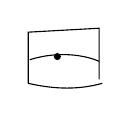
\begin{tikzpicture}[x=1cm,y=1cm]
\draw (0,0) -- (0,0.65) -- (0.9,0.70) -- (0.9,0.05);
\draw (0,0) .. controls (0.35,-0.08) and (0.65,-0.08) .. (0.94,0);
\draw (0.02,0.30) .. controls (0.30,0.39) and (0.64,0.39) .. (0.90,0.28);
\fill (0.37,0.34) circle (0.045);
\end{tikzpicture}}

(iii) Le couple $(\bar X,Y)$ sur $S$ est isomorphe au \deleted{\unsure{couple}} l'image inverse de $(\bar X_0,Y_0)$ sur $S_0$ par $f:S\longrightarrow S_0$.
